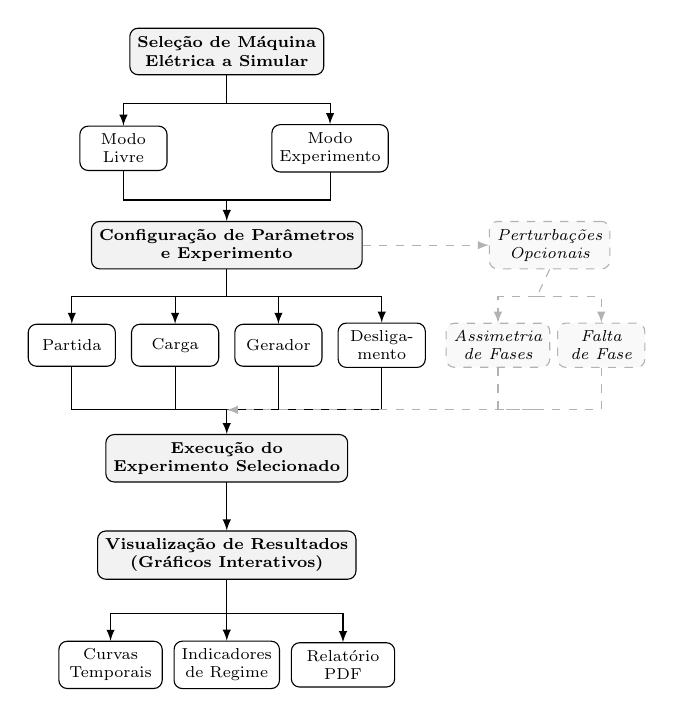
\begin{tikzpicture}[
    scale=0.82, transform shape,
    % Nós comuns
    no/.style={
        draw, rounded corners=3pt, fill=white,
        font=\scriptsize, minimum width=1.35cm,
        minimum height=0.65cm, align=center
    },
    % Nós de destaque
    nodest/.style={
        draw, rounded corners=3pt, fill=gray!10,
        font=\scriptsize\bfseries, minimum width=2.4cm,
        minimum height=0.72cm, align=center
    },
    % Nós opcionais (perturbações)
    noopt/.style={
        draw=gray!60, dashed, rounded corners=3pt, fill=gray!5,
        font=\scriptsize\itshape, minimum width=1.35cm,
        minimum height=0.65cm, align=center
    },
    linha/.style={draw, thin, -latex},
    lopt/.style={draw=gray!60, thin, dashed, -latex}
]

% ---- NÍVEL 0: RAIZ ----
\node[nodest] (raiz) at (0, 0) {Seleção de Máquina\\Elétrica a Simular};

% ---- NÍVEL 1: MODOS ----
\node[no] (m_livre) at (-1.6, -1.5) {Modo\\Livre};
\node[no] (m_exp)   at ( 1.6, -1.5) {Modo\\Experimento};

\coordinate (bif_modo) at (0, -0.8);
\draw[thin]  (raiz.south)   -- (bif_modo);
\draw[linha] (bif_modo) -| (m_livre.north);
\draw[linha] (bif_modo) -| (m_exp.north);

% ---- NÍVEL 2: CONFIGURAÇÃO ----
\node[nodest] (config) at (0, -3.0) {Configuração de Parâmetros\\e Experimento};

\coordinate (merge_modo) at (0, -2.3);
\draw[thin]  (m_livre.south) |- (merge_modo);
\draw[thin]  (m_exp.south)   |- (merge_modo);
\draw[linha] (merge_modo) -- (config.north);

% ---- PERTURBAÇÕES OPCIONAIS (Limpo e Alinhado) ----
\node[noopt] (perturb) at (5, -3.0)  {Perturbações\\Opcionais};
\node[noopt] (p_assim)  at (4.2, -4.55) {Assimetria\\de Fases};
\node[noopt] (p_falta)  at (5.8, -4.55) {Falta\\de Fase};

\draw[lopt] (config.east) -- (perturb.west);

% Bifurcação das perturbações alinhada ao centro do nó pai
\coordinate (bif_p) at (4.8, -3.8); 
\draw[draw=gray!60, thin, dashed] (perturb.south) -- (bif_p);
\draw[lopt] (bif_p) -| (p_assim.north);
\draw[lopt] (bif_p) -| (p_falta.north);

% Merge das perturbações alinhado para evitar linhas duplas
\coordinate (merge_p) at (4.8, -5.55);
\draw[draw=gray!60, thin, dashed] (p_assim.south) |- (merge_p);
\draw[draw=gray!60, thin, dashed] (p_falta.south) |- (merge_p);

% ---- NÍVEL 3: GRUPOS DE EXPERIMENTOS ----
\node[no] (g1) at (-2.4, -4.55) {Partida};
\node[no] (g2) at (-0.8, -4.55) {Carga};
\node[no] (g3) at ( 0.8, -4.55) {Gerador};
\node[no] (g4) at ( 2.4, -4.55) {Desliga-\\mento};

\coordinate (bif_e) at (0, -3.8);
\draw[thin]  (config.south) -- (bif_e);
\draw[linha] (bif_e) -| (g1.north);
\draw[linha] (bif_e) -| (g2.north);
\draw[linha] (bif_e) -| (g3.north);
\draw[linha] (bif_e) -| (g4.north);

% ---- NÍVEL 4: EXECUÇÃO ----
\node[nodest] (sim) at (0, -6.3) {Execução do\\Experimento Selecionado};

\coordinate (merge_e) at (0, -5.55);
\draw[thin]  (g1.south) |- (merge_e);
\draw[thin]  (g2.south) |- (merge_e);
\draw[thin]  (g3.south) |- (merge_e);
\draw[thin]  (g4.south) |- (merge_e);
\draw[linha] (merge_e)  -- (sim.north);

% Conexão única vinda do bloco de perturbações
\draw[lopt] (merge_p) -- (merge_e);

% ---- NÍVEL 5: VISUALIZAÇÃO ----
\node[nodest] (vis) at (0, -7.8) {Visualização de Resultados\\(Gráficos Interativos)};
\draw[linha] (sim.south) -- (vis.north);

% ---- NÍVEL 6: SAÍDAS ----
\node[no, minimum width=1.6cm] (a1) at (-1.8, -9.5) {Curvas\\Temporais};
\node[no, minimum width=1.6cm] (a2) at ( 0.0, -9.5) {Indicadores\\de Regime};
\node[no, minimum width=1.6cm] (a3) at ( 1.8, -9.5) {Relatório\\PDF};

\coordinate (bif_a) at (0, -8.7);
\draw[thin]  (vis.south) -- (bif_a);
\draw[linha] (bif_a) -| (a1.north);
\draw[linha] (bif_a) -- (a2.north);
\draw[linha] (bif_a) -| (a3.north);

\end{tikzpicture}